\section{I/O Processing Schemes}
\label{sec:io_processing}

This section presents a new zero-copy I/O processing scheme for GPU
computing, which differs from existing schemes in that both GPU
execution and data transfer times are minimized to achieve the goal of
low-latency GPU computing. 
In the rest of this section, we first investigate two existing schemes,
{\hd} and {\hp}, that are already supported by CUDA.
We then present a new scheme called {\dm} and introduce a hybrid
variant of {\dm} and an existing one, suited for a specific case. 

\subsection{Host and Device Memory ({\hd})}
\label{sec:hd}

\begin{figure}[!t]
 \centering
 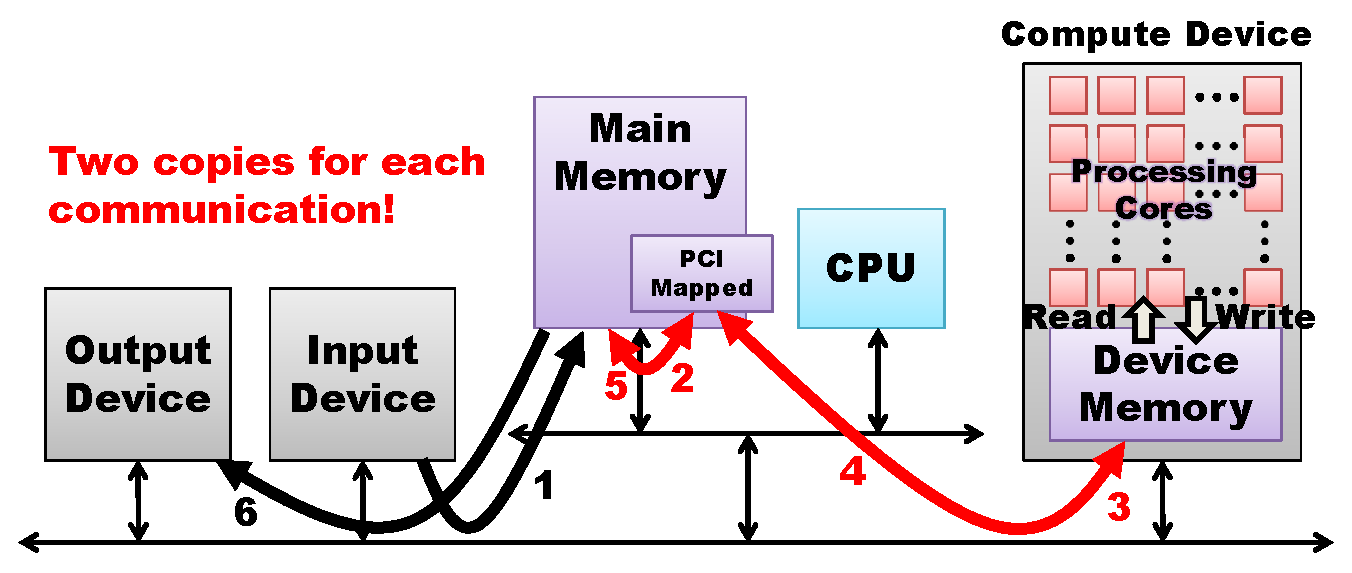
\includegraphics[width=\hsize]{eps/hd2.eps}
 \caption{The traditional {\hd} scheme.}
 \label{fig:hd}
\end{figure}

This is the most common scheme of GPU computing in the literature.
In this scheme, there is space overhead in that the input and output
data exist in both the device and the host memory at the same time and
must be explicitly copied between them.
Furthermore, there is a time penalty incurred to copy data at a cost
nearly proportional to the data size.
When applying this scheme, we allocate the same size of buffers to the
host and the device memory individually and copy data between them
explicitly.

Figure~\ref{fig:hd} illustrates an overview of how this scheme works:
\begin{enumerate} \itemsep1pt
 \item The device driver of the input device configures the input device
       to send data to the allocated space of the host memory.
 \item The device driver of the GPU copies the data to the
       PCI-mapped space of the host memory, which is accessible to the
       device memory.
 \item The device driver of the GPU further copies the data to the
       allocated space of the device memory.
       Now, the GPU can access the data.
 \item When GPU computation is completed, the device driver of the
       GPU copies the output data back to the PCI-mapped space of the
       host memory.
 \item The device driver of the GPU further copies the output data back
       to the allocated space of the host memory.
 \item Finally, the device driver of the output device configures the
       output device to receive the data from the allocated space of the
       host memory.
\end{enumerate}

As described above, the {\hd} scheme incurs overhead to copy the same
data twice for each direction of data transfer between the host and the
device memory.
This overhead might be a crucial penalty for low-latency GPU computing.

\subsection{Host Pinned Memory ({\hp})}
\label{sec:hp}

\begin{figure}[!t]
 \centering
 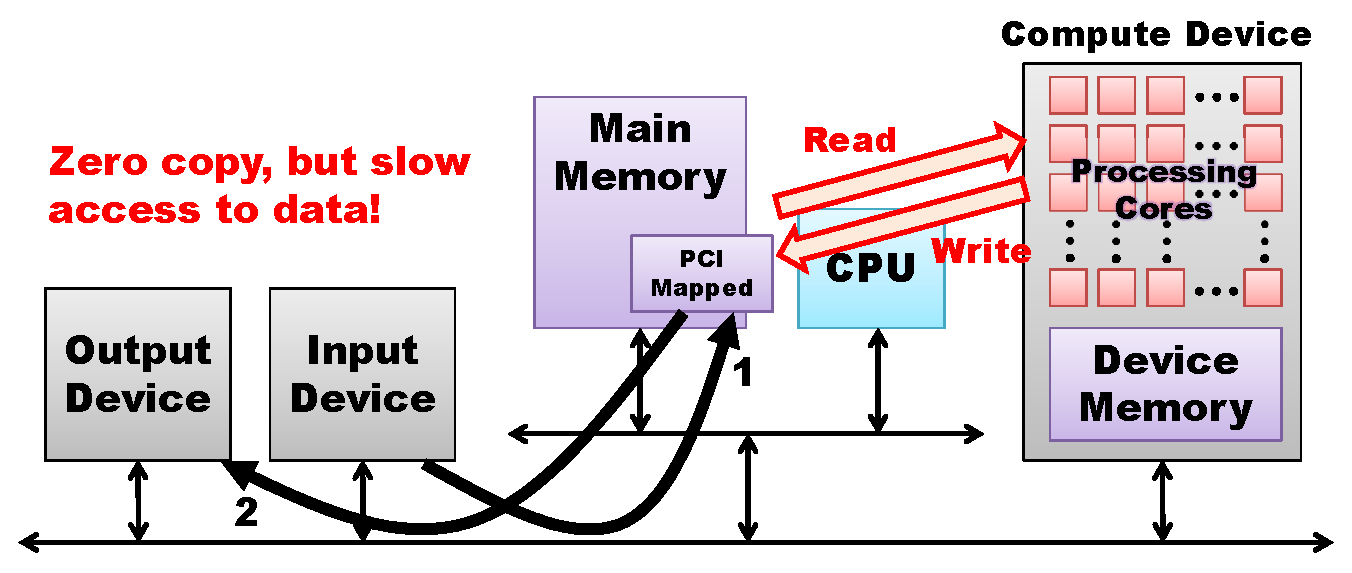
\includegraphics[width=\hsize]{eps/hp2.eps}
 \caption{The traditional {\hp} scheme.}
 \label{fig:hp}
\end{figure}

As an alternative to allocating the buffers to both the host and the
device memory, we can allocate the buffers to page-locked PCI-mapped
space of the host memory, also known as \textit{pinned} host memory.
Since recent GPU architectures support unified addressing, this memory
space can be referenced by the GPU.
A major advantage of this scheme is that the input and the output
devices can also directly access this memory space, which means that
there is no need for intermediate buffers and data copies to have the
GPU access the data.

Figure~\ref{fig:hp} illustrates an overview of how this scheme works.
Unlike the {\hd} scheme, the data transfer flow is pretty simple.
There are no additional data copies required, since PCI-mapped space is
directly accessible to the input and the output devices.
It is also pinned to always reside in the host memory, and therefore the
GPU can read and write the data directly.
However, this data access is expensive as it is a PCIe communication.

\subsection{Device Memory Mapped to Host ({\dm})}
\label{sec:dm}

\begin{figure}[!t]
 \centering
 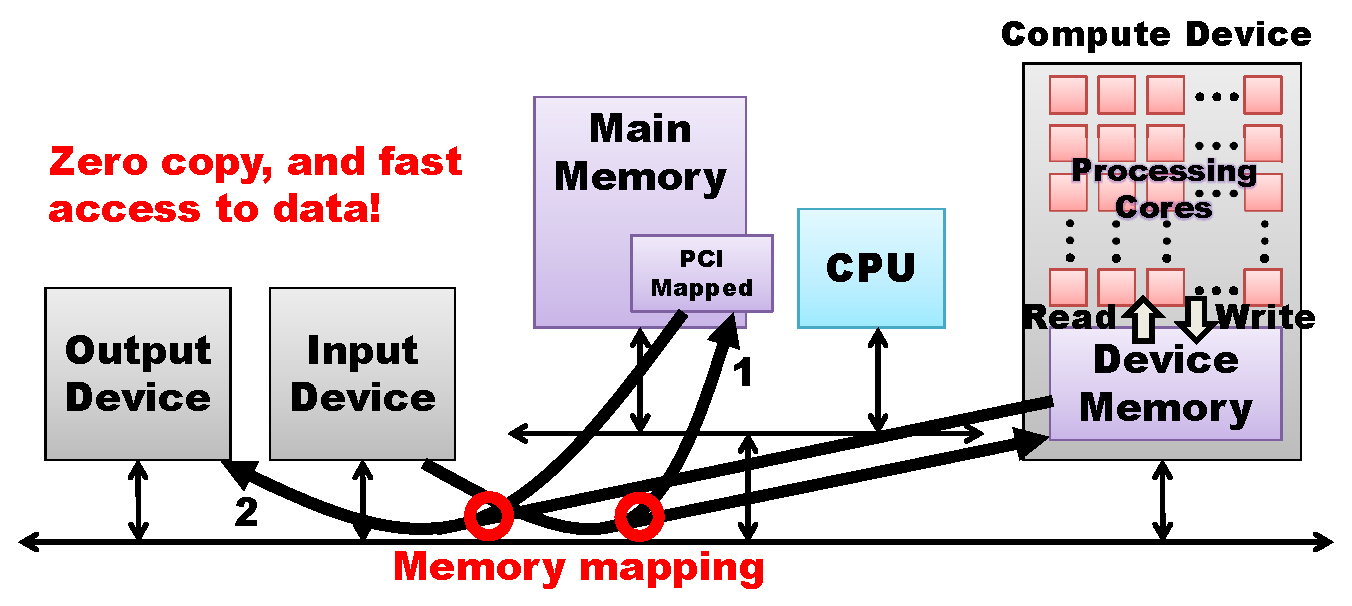
\includegraphics[width=\hsize]{eps/dm2.eps}
 \caption{The new zero-copy {\dm} scheme.}
 \label{fig:dm}
\end{figure}

We now present {\dm}, which overcomes the problems of the {\hd} and the
{\hp} schemes.
The key to the {\dm } scheme is having the PCIe BAR point to the
allocated space of the device memory, while mapping the allocated space
of the host memory to the PCIe BAR as well.
As a result, when the input device sends data to the PCI-mapped space of
the host memory, the data seamlessly appear on the corresponding
allocated space of the device memory.
This scheme, hence, does not require the CPU to intermediate to copy the
data between the host and the device memory, which removes the latency
of data transfer observed in the {\hd} scheme.
On the other hand, it also maintains the performance benefit of having
the data on board, solving the problem of slow data accesses faced in
the {\hp} scheme.

Assuming that some space is already allocated to the device
memory, the system is required to support the following functions to have I/O
devices directly access this memory space:

\begin{itemize} \itemsep1pt
 \item \textbf{Mapping Memory:}
       As technology reads today, PCIe BARs are the most reasonable
       windows that see through the device memory from the host and I/O
       space.
       Therefore, we first need to reserve the corresponding size of
       PCIe BAR space, and next map it to the allocated space of the
       device memory.
       Now, if the user requests to access it from the host program, the
       system needs to further remap it to the user buffers.
 \item \textbf{Unmapping Memory:}
       PCIe BARs are limited resources. Most GPUs currently provide at
       most 128MB for a single BAR.
       Therefore, unmapping the device memory from the BAR is an essential
       function for this scheme.
 \item \textbf{Getting Physical Address:}
       The mapped space is typically referenced as virtual memory space
       of the GPU or the CPU.
       However, I/O devices often target physical address for data transfer.
       Hence, the system needs to maintain the physical address of the
       PCI-mapped space, and relay it to the device drivers of I/O devices.
\end{itemize}

In fact, PCIe BARs are not only the windows that can communicate with
the device memory.
Recent GPUs support special windows upon the memory-mapped I/O (MMIO) space.
To simplify the discussion, this paper focuses on PCIe BARs, but the
same concept of zero-copy I/O processing can be also applied to any
mapping method.

\subsection{Device Memory Mapped Hybrid ({\dmh})}
\label{sec:dmh}

This is a hybrid of the {\dm} and the {\hd} schemes, which is in
particular suited to communicate between the host and the device
memory.
Applications of CPS using I/O devices, thereby, may not benefit from
this scheme; if the host memory is used to store some data, this scheme
is still effective.

This scheme is the same as {\dm} as far as memory allocation
and mapping.
For transferring data from the host to the device memory, we have the
host processor reference the device memory directly through the
mapped region, like the {\dm} scheme.
However, we perform an explicit copy from the device to the host memory
for an opposite direction of data transfer.
The motivation to do so is that writing to the host memory is more
expensive than reading, due to functionality of the host memory
management unit (MMU).
We evaluate the impact of this scheme in Section~\ref{sec:benchmarking}.
